\section{第二章 逻辑代数基础 作业}

\subsection{题2.2 证明下列逻辑恒等式}
\begin{enumerate}
    \item $AB' + B + A'B = A + B$

    \textbf{证明：}
    \begin{align*}
    \text{左边} &= AB' + B + A'B \\
              &= AB' + B(1 + A') \\
              &= AB' + B \\
              &= A + B = \text{右边}
    \end{align*}

    \item $(A + C')(B + D)(B + D') = AB + BC'$

    \textbf{证明：}
    \begin{align*}
    \text{左边} &= (A + C') \cdot \big[(B + D)(B + D')\big] \\
              &= (A + C') \cdot B \\
              &= AB + BC' = \text{右边}
    \end{align*}

    \item $A'B'C' + A(B + C) + BC = (AB'C' + A'B'C + A'BC')'$

    \textbf{证明：}
    \begin{align*}
    \text{右边} &= (AB'C')'(A'B'C)'(A'BC')' \\
                &= (A' + B + C)(A + B + C')(A + B' + C) \\
                &= A'B'C' + AB + AC + BC \\
                &= A'B'C' + A(B + C) + BC = \text{左边}
    \end{align*}
\end{enumerate}

\subsection{题2.6 写出图P2.6(a)(b)的输出逻辑函数式}
\begin{figure}[ht]
    \centering
    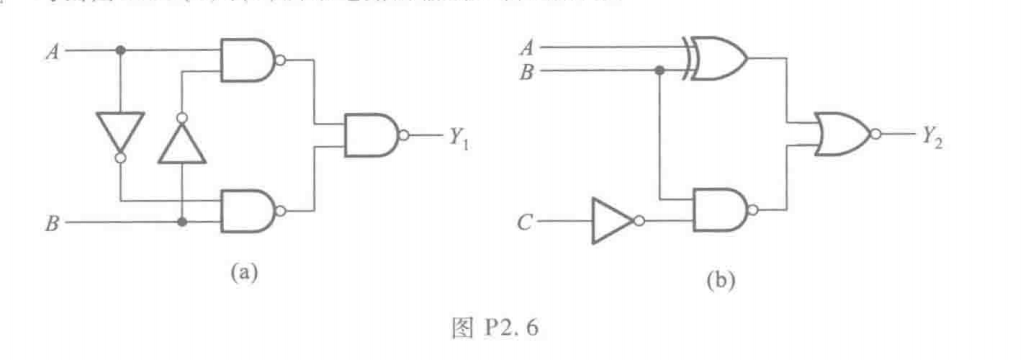
\includegraphics[width=0.8\textwidth]{2.6.png}
    \caption{图P2.6 逻辑电路图}
\end{figure}

\textbf{解：}
\begin{align*}
Y_a &= \overline{\overline{A\cdot B'} \cdot \overline{A'\cdot B}} = A \oplus B \\
Y_b &= \overline{(A\oplus B) + \overline{B C'}} = AB\overline{C}
\end{align*}

\subsection{题2.8 根据波形图写出真值表与逻辑函数式}
\begin{figure}[ht]
    \centering
    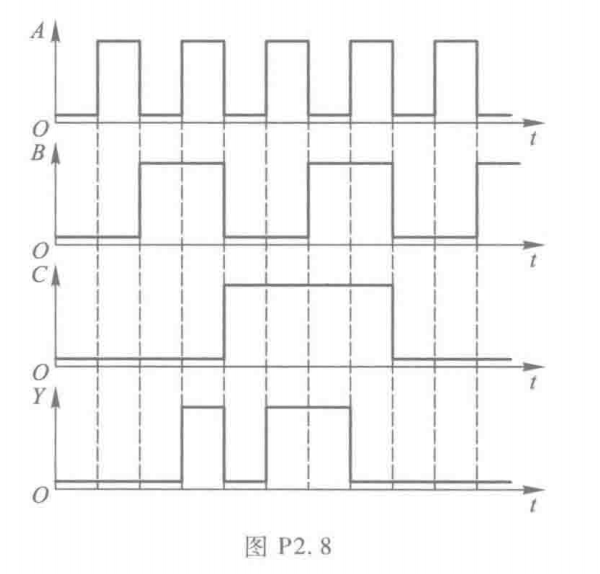
\includegraphics[width=0.8\textwidth]{2.8.png}
    \caption{图P2.8 波形图}
\end{figure}

\textbf{解：}
由波形图可得
\[
Y = \sum m(3,6) = A'BC + ABC'
\]

\subsection{题2.10 化为最小项之和形式}
\begin{enumerate}
    \item $Y = A'BC + AC + B'C$

    \textbf{解：}
    \begin{align*}
    Y &= A'BC + AC(B+B') + B'C(A+A') \\
      &= A'BC + ABC + AB'C + A'B'C \\
      &= \sum m(1,3,6,7)
    \end{align*}

    \item $Y = AB'C'D + BCD + A'D$

    \textbf{解：}
    \begin{align*}
    Y &= AB'C'D + BCD(A+A') + A'D(B+B')(C+C') \\
      &= \sum m(1,3,5,7,9,15)
    \end{align*}

    \item $Y = A + B + CD$

    \textbf{解：}
    \[
    Y = \sum m(3,4,5,6,7,8,9,10,11,12,13,14,15)
    \]

    \item $Y = AB + ((BC)'(C' + D'))'$

    \textbf{解：}
    \begin{align*}
    Y &= AB + BC + CD \\
      &= \sum m(3,6,7,11,12,13,14,15)
    \end{align*}
\end{enumerate}

\subsection{题2.12 化简逻辑函数}
\begin{enumerate}
    \item $ACD' + D'$

    \textbf{解：}
    \[
    Y = D'(AC + 1) = D'
    \]

    \item $AB' + AC + BC$

    \textbf{解：}
    \[
    Y = AB' + BC
    \]

    \item $E'F' + E'F + EF' + EF$

    \textbf{解：}
    \[
    Y = E'(F'+F) + E(F'+F) = E' + E = 1
    \]

    \item $A'BC + (A + B')C$

    \textbf{解：}
    \[
    Y = A'BC + AC + B'C = C(A'B + A + B') = C
    \]
\end{enumerate}

\subsection{题2.13 化为最简与或式}
\begin{enumerate}
    \item $Y = AB'C + A' + B + C'$

    \textbf{解：}
    \[
    Y = A' + B + C' + AB'C = A' + B + C' + C = 1
    \]

    \item $Y = AB'CD + ABD + AC'D$

    \textbf{解：}
    \[
    Y = AD(B'C + B + C') = AD
    \]

    \item $Y = AC(C'D + A'B) + BC((B' + AD)' + CE)'$

    \textbf{解：}
    \begin{align*}
    Y &= AC'D + ABCD(C' + E') \\
      &= AC'D
    \end{align*}

    \item $Y = A + (B + C')'(A + B' + C)(A + B + C)$

    \textbf{解：}
    \begin{align*}
    Y &= A + B'C(A + C) \\
      &= A + B'C
    \end{align*}

    \item $Y = AC + AC'D + AB'E'F + B(D \oplus E) + BC'DE' + BC'D'E + ABE'F$

    \textbf{解：}
    \begin{align*}
    Y &= A(C + C'D) + AE'F + B(D \oplus E)(1 + C') \\
      &= AC + AD + AE'F + B(D \oplus E)
    \end{align*}
\end{enumerate}

\subsection{题2.15 卡诺图化简}
\begin{enumerate}
    \item $Y_1 = C + ABC$

    \textbf{解：}
    \[
    Y_1 = C(1 + AB) = C
    \]

    \item $Y_2 = AB'C + BC + A'BC'D$

    \textbf{解：}
    \[
    Y_2 = C
    \]

    \item $Y_3(A,B,C) = \sum m(1,2,3,7)$

    \textbf{解：}
    \[
    Y_3 = A'C + BC
    \]

    \item $Y_4(A,B,C,D) = \sum m(0,1,2,3,4,6,8,9,10,11,14)$

    \textbf{解：}
    \[
    Y_4 = B' + CD'
    \]
\end{enumerate}

\subsection{题2.16 卡诺图化简}
\begin{enumerate}
    \item $Y = AB' + A'C + BC + C'D$

    \textbf{解：}
    \[
    Y = A'C + AB' + C'D
    \]

    \item $Y = A'B' + BC' + A' + B' + ABC$

    \textbf{解：}
    \begin{align*}
    Y &= A'(1 + B') + B'(1 + A) + BC' + ABC \\
      &= A' + B' + C
    \end{align*}
\end{enumerate}

\subsection{题2.18 写出逻辑式并化简}
\begin{figure}[ht]
    \centering
    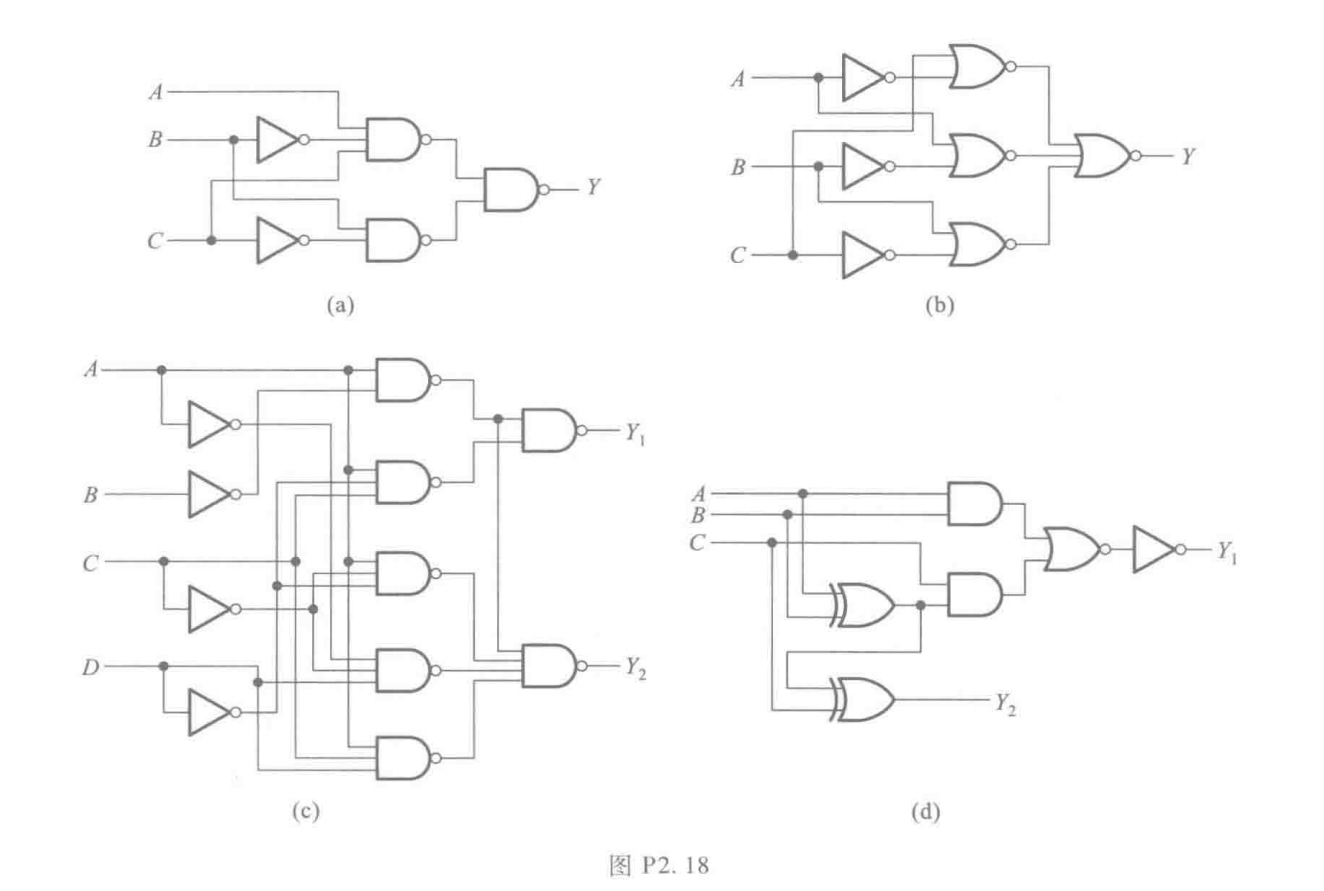
\includegraphics[width=0.85\textwidth]{2.18.png}
    \caption{图P2.18 逻辑图}
\end{figure}

\textbf{解：}
\begin{align*}
Y_a &= A\overline{B} + \overline{C} \\
Y_b &= \overline{B} + AC \\
Y_c &= AC + \overline{B}D
\end{align*}

\subsection{题2.20 (1) 带约束项化简}
\[
Y_1 = AB'C' + ABC + A'B'C + A'BC',\quad A'B'C' + A'BC = 0
\]

\textbf{解：}
利用约束项合并卡诺图：
\[
Y_1 = AC + B'C'
\]

\subsection{题2.21 (1)(3) 带无关项化简}
\begin{enumerate}
    \item $Y_1 = \sum m(0,1,2,4) + d(5,6)$

    \textbf{解：}
    \[
    Y_1 = A' + B'C'
    \]

    \item $Y_3 = \sum m(3,5,6,7,10) + d(0,1,2,4,8)$

    \textbf{解：}
    \[
    Y_3 = A'B + AC + A'D
    \]
\end{enumerate}

\subsection{题2.24 多输出函数化简}
\begin{align*}
Y_1 &= \sum m(0,1,8,9,10,12,13,14) \\
Y_2 &= \sum m(0,1,2,3,6,7,10,14)
\end{align*}

\textbf{解：}
\[
Y_1 = B'C' + AC' + ABD',\quad
Y_2 = A'B' + A'C + BC'D'
\]

\subsection{题2.26 化为与非–与非式}
\begin{enumerate}
    \item $Y = AB + BC + AC$

    \textbf{解：}
    \[
    Y = \overline{\overline{AB} \cdot \overline{BC} \cdot \overline{AC}}
    \]

    \item $Y = (A' + B)(A + B')C + (BC)'$

    \textbf{解：}
    \begin{align*}
    Y &= AB'C + A'BC + B' + C' \\
      &= B' + C' = \overline{\overline{B'} \cdot \overline{C'}}
    \end{align*}

    \item $Y = (ABC' + AB'C + A'BC)'$

    \textbf{解：}
    \[
    Y = \overline{\overline{ABC'} \cdot \overline{AB'C} \cdot \overline{A'BC}}
    \]

    \item $Y = A(BC)' + ((AB')' + A'B' + BC)'$

    \textbf{解：}
    \begin{align*}
    Y &= AB' + AC' \\
      &= \overline{\overline{AB'} \cdot \overline{AC'}}
    \end{align*}
\end{enumerate}